\subsection{Estimation of events with electrons faking photons}

The fake-rate estimation predicts the expected rate from $W(e\nu)$ 
events where the electron fakes a photon.  The method relies on
computing an $e\rightarrow\gamma$ fake rate, derived from a mixture
of simulation and data, and applying the fake rate as an event weight
to the single electron control region, in which we veto events with
a photon.  

The kinematic selection for the single electron control region is exactly the 
same as the single photon control region except that we require exactly 
zero photons, exactly one electron with tight ID criteria, and use the tight electron
4-vector in place of the photon 4-vector where relevant. 

The crux of this method is the derivation of the fake rate.  The fake
rate in a given region of phase space is defined to be the ratio of events 
with photons and no electron with respect 
to events with exactly one tight electron and zero photons.  The 
fake rate will be derived using simulated W/$t\bar{t}$ events.  
However, due to MC modeling of various nuisances relevant to electron
reconstruction, an overall difference is to be expected between 
data and MC fake-rates.  To correct for this, we will also 
measure the fake-rate in data and MC using DY events with a 
tag-and-probe (T\&P) method.  These T\&P measurements will be 
used to correct the fake rates derived on W/$t\bar{t}$ simulations.

The overall prediction is then given by:
\begin{equation} \label{eqn:fake_pred}
  N_{e\rightarrow\gamma} = N_{e}^{data} \cdot f^{tt,W} \cdot \beta^{data/MC} \cdot \frac{\epsilon^{trig}_{SR}}{\epsilon^{trig}_{CR}},
\end{equation}
where $f^{tt,W}$ is the fake-rate derived from W/$t\bar{t}$ simulation, 
$\beta$ represents the T\&P corrections factors, and $\epsilon$ represents 
the measured trigger efficiency.

There are two important paramterizations, namely, $f^{tt,W}$ and $\beta$.  

\subsubsection{Fake-rate parameterization}

The fake rate is parameterized as a function of local metrics relevant to electron reconstruction;
the electron \pt and the charged track multiplicity, $Q_{mult}$ around the electron 
are found to give the best closure on MC.  The metric $Q_{mult}$ 
is defined to be the sum of charged PF candidates with the jet 
matched, $\dR<0.3$, to the electron. Since we require electrons have at least
$\pt>100~\gev$, the jet clustering algorithm almost always clusters
the electron into an AK4 jet.  On the rare occasions that there is 
no matched jet, the event is rejected.  The distribution of $Q_{mult}$
is shown in Figure~\ref{fig:qMultDist} for DY, W+jets, and $t\bar{t}$ events. 

\begin{figure}[h!]
\centering
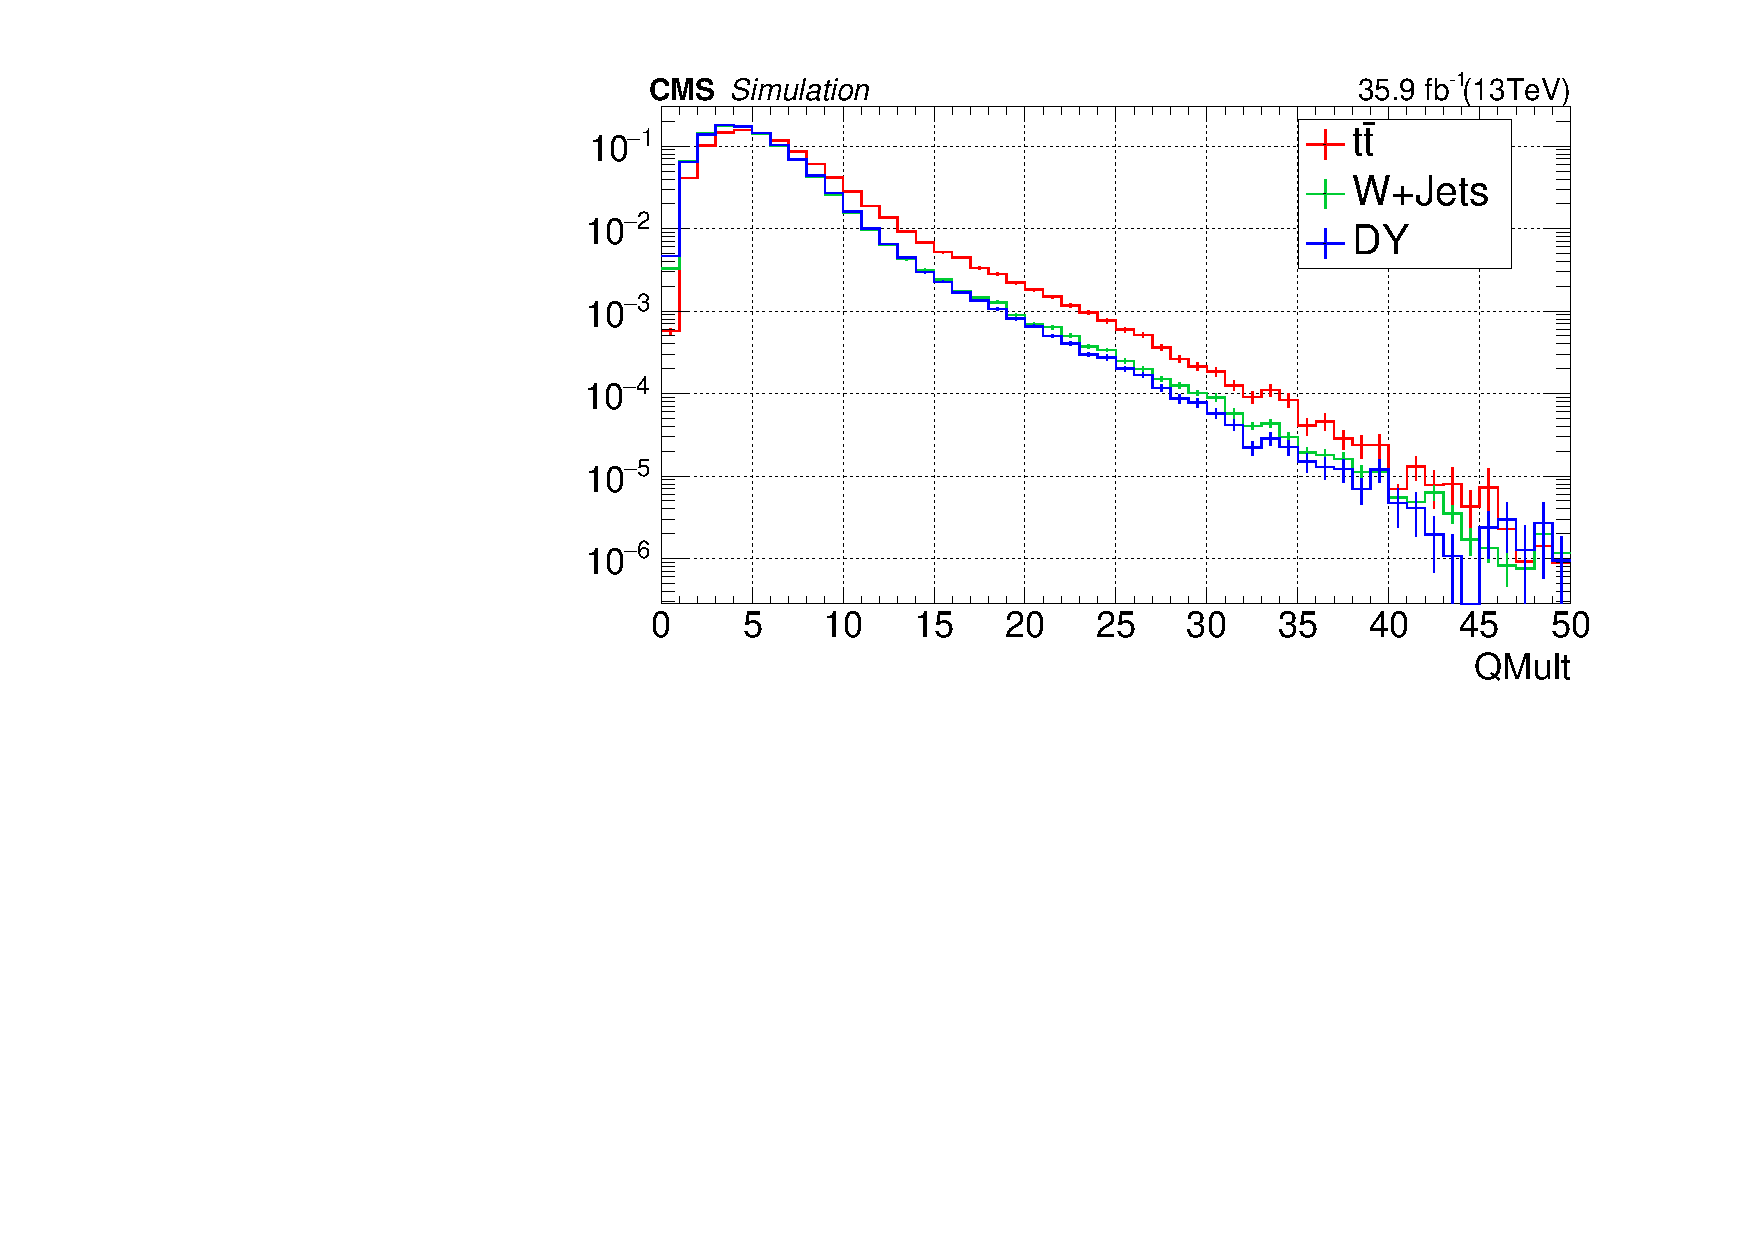
\includegraphics[width=0.48\linewidth]{../Figures/Chap3/fake_rate_closure/QMult_eleJet_ttwDY.pdf}
\caption[$Q_{mult}$ distribution for DY, W+jets, and $t\bar{t}$]{$Q_{mult}$ distribution in a jet matched to the electron in 
DY, W+jets, and $t\bar{t}$ events. Each of these distribution are scaled to unit area.}
\label{fig:qMultDist}
\end{figure}

When deriving the fake-rate from simulation events are divided into
two categories, signal region (SR) events, and control region (CR) events.  Signal region events are 
those with zero electrons found and an EM objects matched, $\dR<0.2$, to a gen-level
electron. Control region events are those with 1 tight electron ($\pt>100~gev$), 
exactly zero photons, and $m_T(e,\ptmiss)<100~\gev$; the last requirement 
increases the purity of the control sample and avoids overlap with 
signal events.  After these selections are applied, the fake rate is then
defined as $f^{tt,W}=N_{SR}/N_{CR}$.  

Table~\ref{tab:fakeRateParam} shows the parameterization
of the fake rate that is used.   To validate this parameterization, the
fake rate method is applied to MC and the prediction is compared to the 
true yields from simulation.  Figure~\ref{fig:fakeRateClosure} show the comparison 
of the prediction (applying the fake rate parameterization to single 
electron MC events) and true yields; the agreement is found to be 
within 20\%.
                            

\begin{figure}[h!]                           
\centering
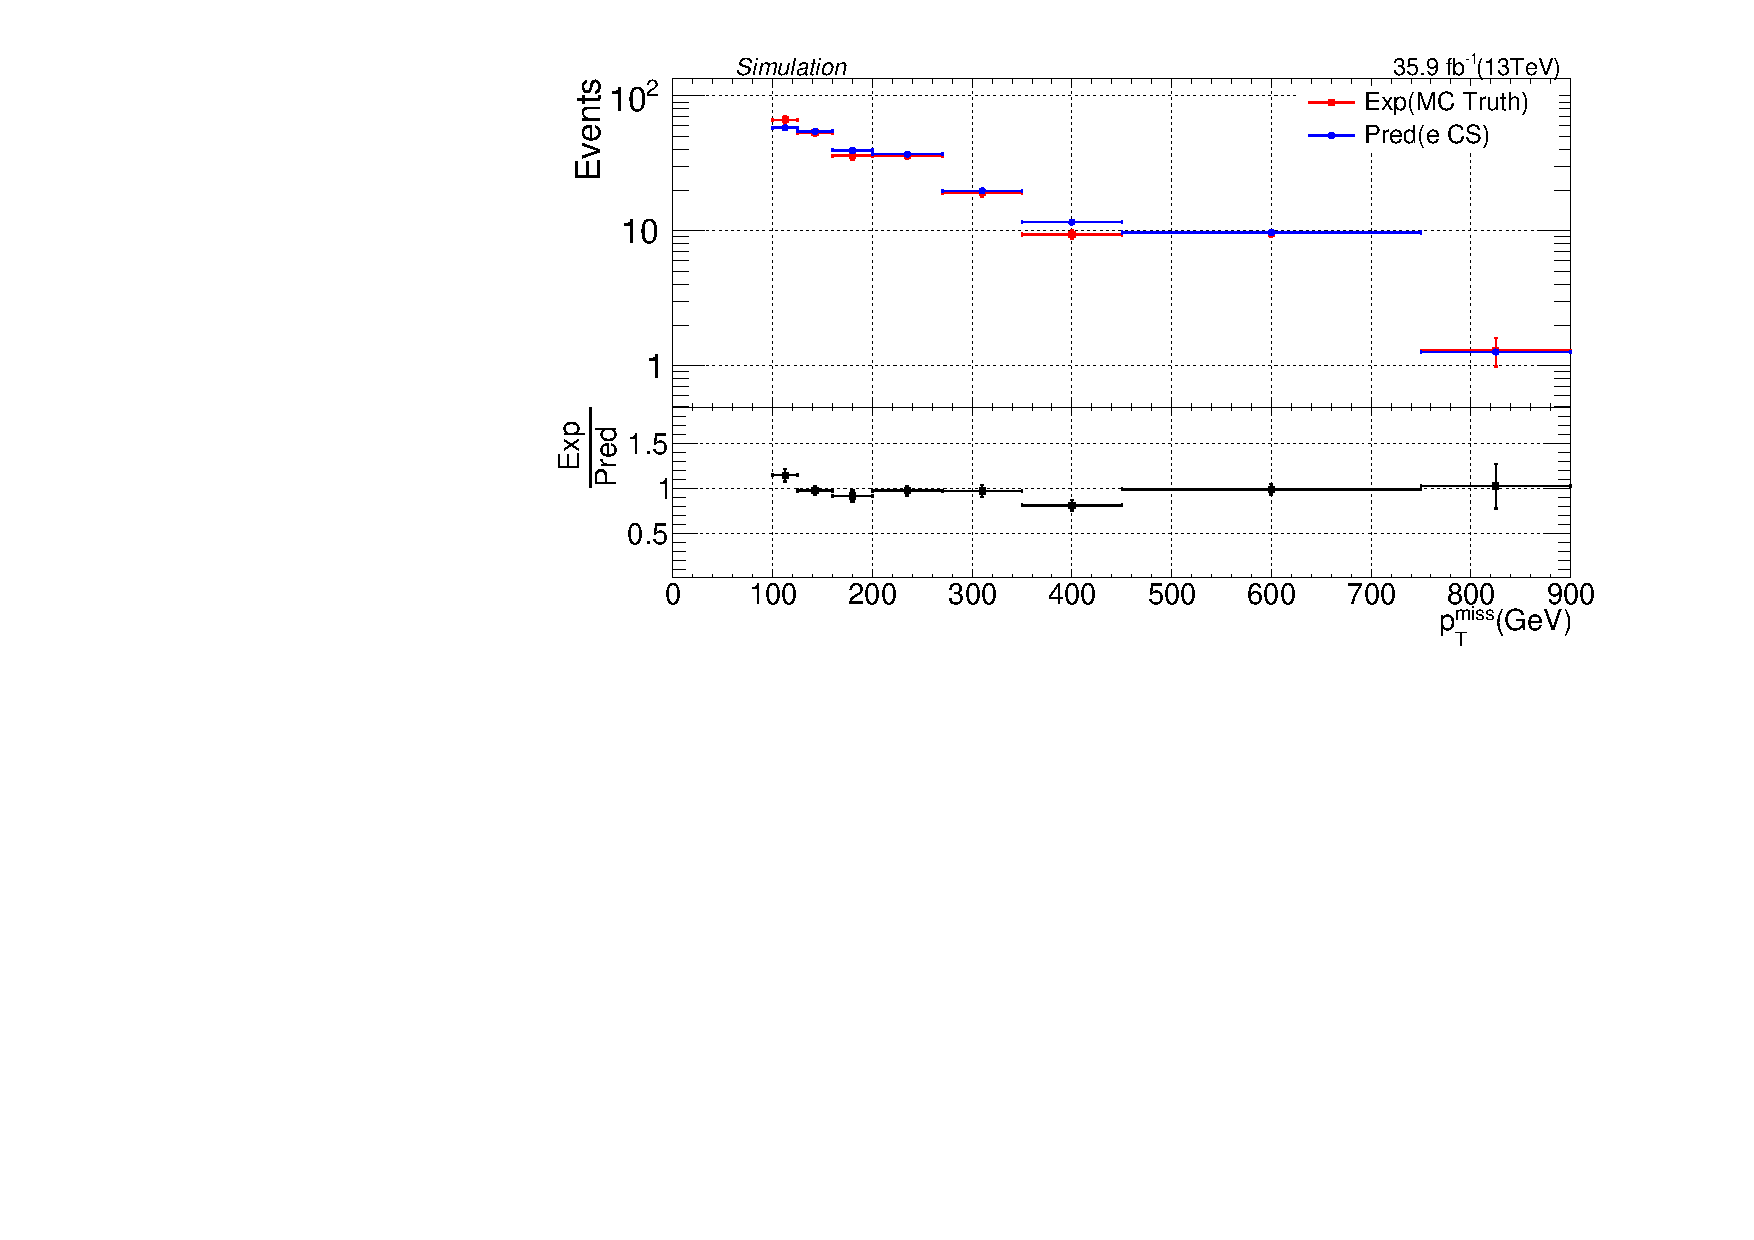
\includegraphics[width=0.48\linewidth]{../Figures/Chap3/fake_rate_closure/fakeRateClosure_met.pdf}
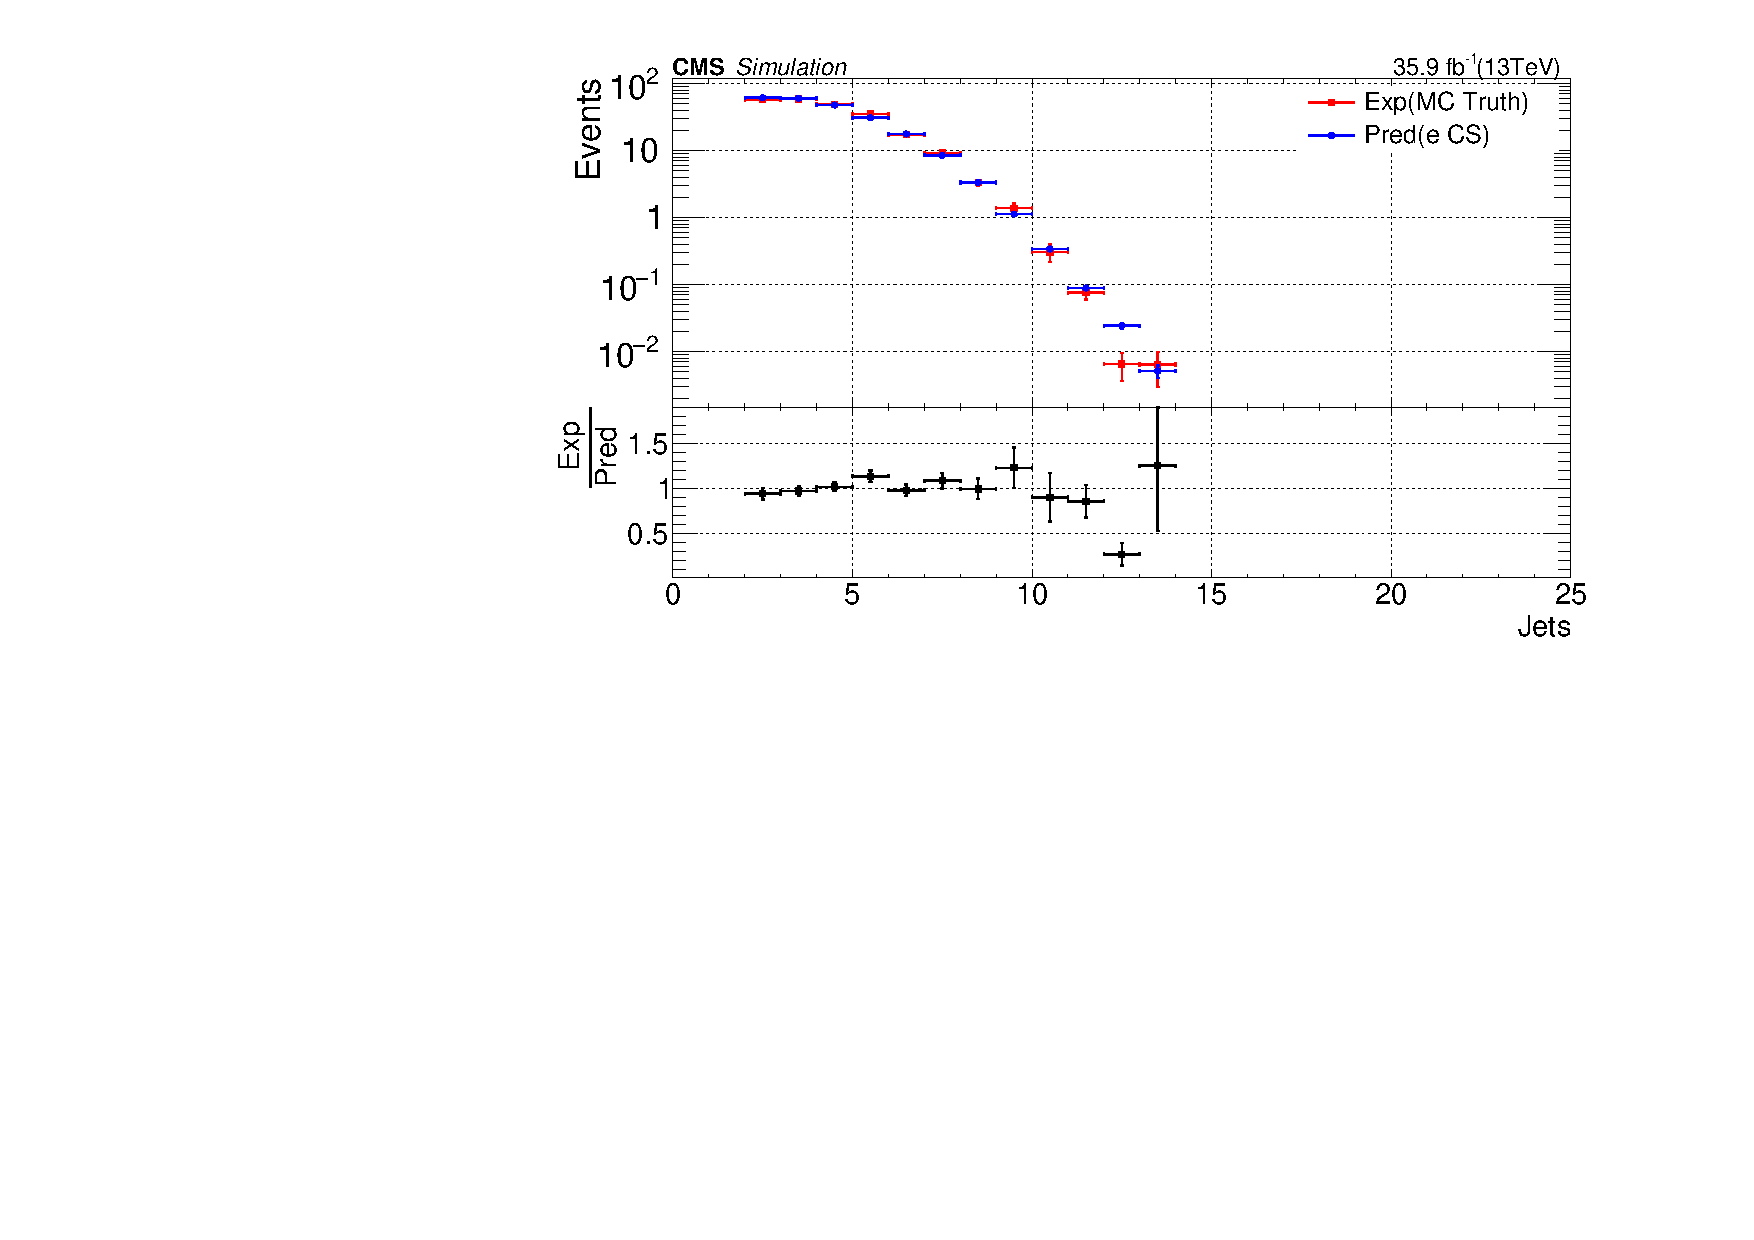
\includegraphics[width=0.48\linewidth]{../Figures/Chap3/fake_rate_closure/fakeRateClosure_njets.pdf}\\
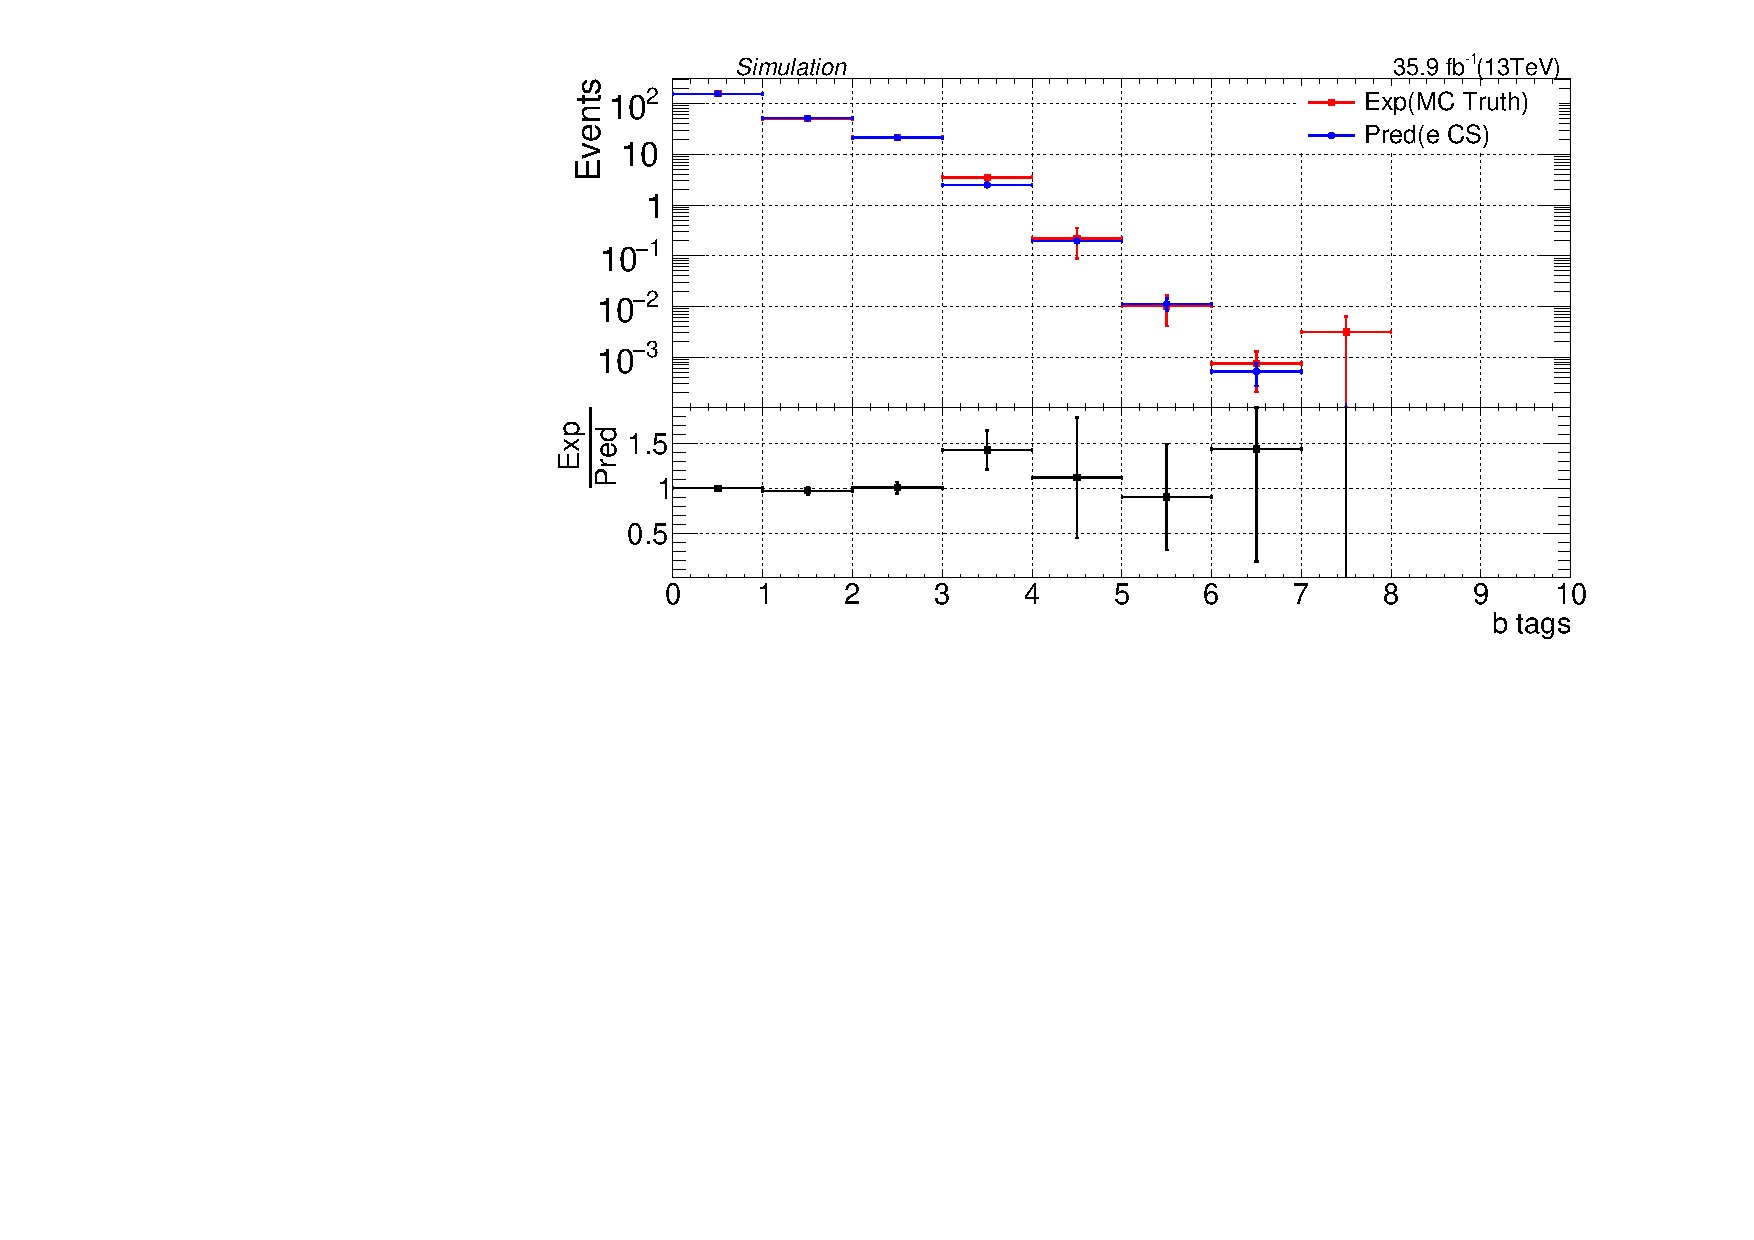
\includegraphics[width=0.48\linewidth]{../Figures/Chap3/fake_rate_closure/fakeRateClosure_btags.pdf}
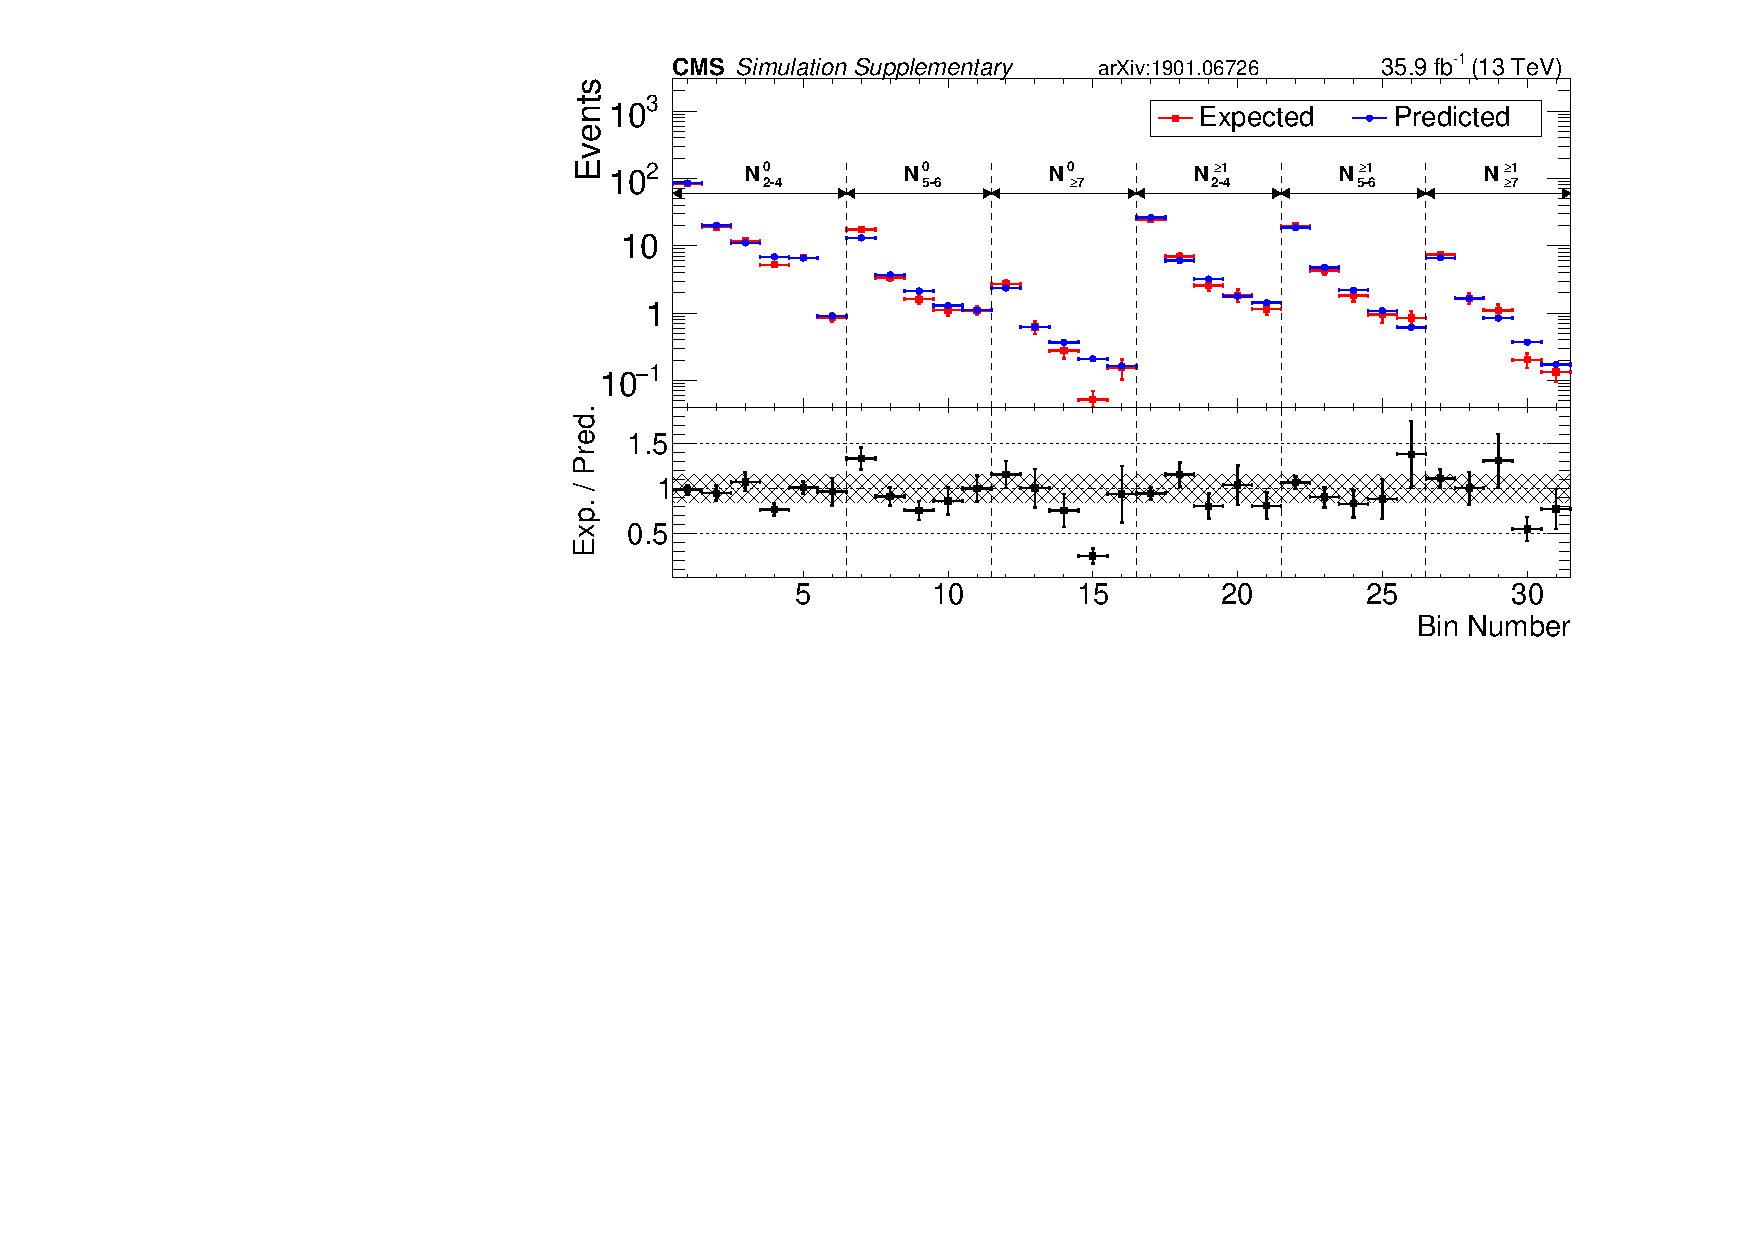
\includegraphics[width=0.48\linewidth]{../Figures/Chap3/anaPublic/fakerateClosure}
\captionsetup{width=.9\linewidth}
\caption[Fake rate closures]{Comparison of fake rate prediction using fake rate parameterization
and true MC yields using $W/t\bar{t}+(\gamma)$ simulations versus \ptmiss (top left), 
\nj (top right), \nb (bottom left) and search bins (bottom right). The hashed region in the lower panel 
of bottom right plot shows the total systematic uncertainty.}
\label{fig:fakeRateClosure}
\end{figure}

\subsubsection{Data/MC fake rate corrections}

The data/MC corrections for the fake rate are computed using a T\&P method on 
Drell-Yan events.  Z bosons are reconstructed using a tag object and a probe object.    
The tag object definition is one tight electron with $\pt>40~\gev$.  The probe
can either be one tight electron or one photon with $\pt>100~\gev$. Event selections
otherwise includes, $\nj\geq2$, $\ptmiss<100~\gev$, zero isolated tracks 
(not including the tag/probe objects), and \dR(tag, probe)$>0.2$. 
In the case where the probe satisfies the tag criteria, the tag is chosen
randomly and the event is counted twice. 

Once the photon and electron candidates are formed, the $m_{\ell\ell}$ distribution
is fit using a Briet-Wigner convoluted with a Gaussian to model the Z boson peak and
a polynomial to model the combinatorial background.  The fit is performed on 
both data and MC in regions of $Q_{mult}$, which is the variable for which 
the discrepancies between data and MC are found to be the largest. Table~\ref{tab:fakeRateCorrections}
shows the fitted fake rate in data and MC, and the corresponding correction
factor in each of the $Q_{mult}$ bins. Figure~\ref{fig:tpFits} shows the 
fit results for each of the fake rate measurements.

\begin{table}[h!]
\centering
\caption[Fake rate SFs]{Fake rate as measured by T\&P procedure on Drell-Yan events in data and MC.}
\label{tab:fakeRateCorrections}
\begin{tabular}{c|c|c|c}
\hline
$Q_{mult}$ & MC fake rate    & data fake rate  & scale factor \\ \hline\hline

0-1        & 0.014 $\pm$ 0.002    & 0.016 $\pm$ 0.003    & 1.17 $\pm$ 0.27  \\ \hline
$\geq$2    & 0.015 $\pm$ 0.001    & 0.018 $\pm$ 0.002    & 1.21 $\pm$ 0.16  \\ \hline
%2-3        & 0.014 $\pm$     & 0.018 $\pm$     & 1.28 $\pm$   \\ \hline
%4-5        & 0.013 $\pm$     & 0.016 $\pm$     & 1.26 $\pm$   \\ \hline
%6-7        & 0.014 $\pm$     & 0.019 $\pm$     & 1.34 $\pm$   \\ \hline
%$\geq$8    & 0.016 $\pm$     & 0.020 $\pm$     & 1.25 $\pm$   \\ \hline
\end{tabular}
\end{table}

\begin{figure}[h!]
\centering
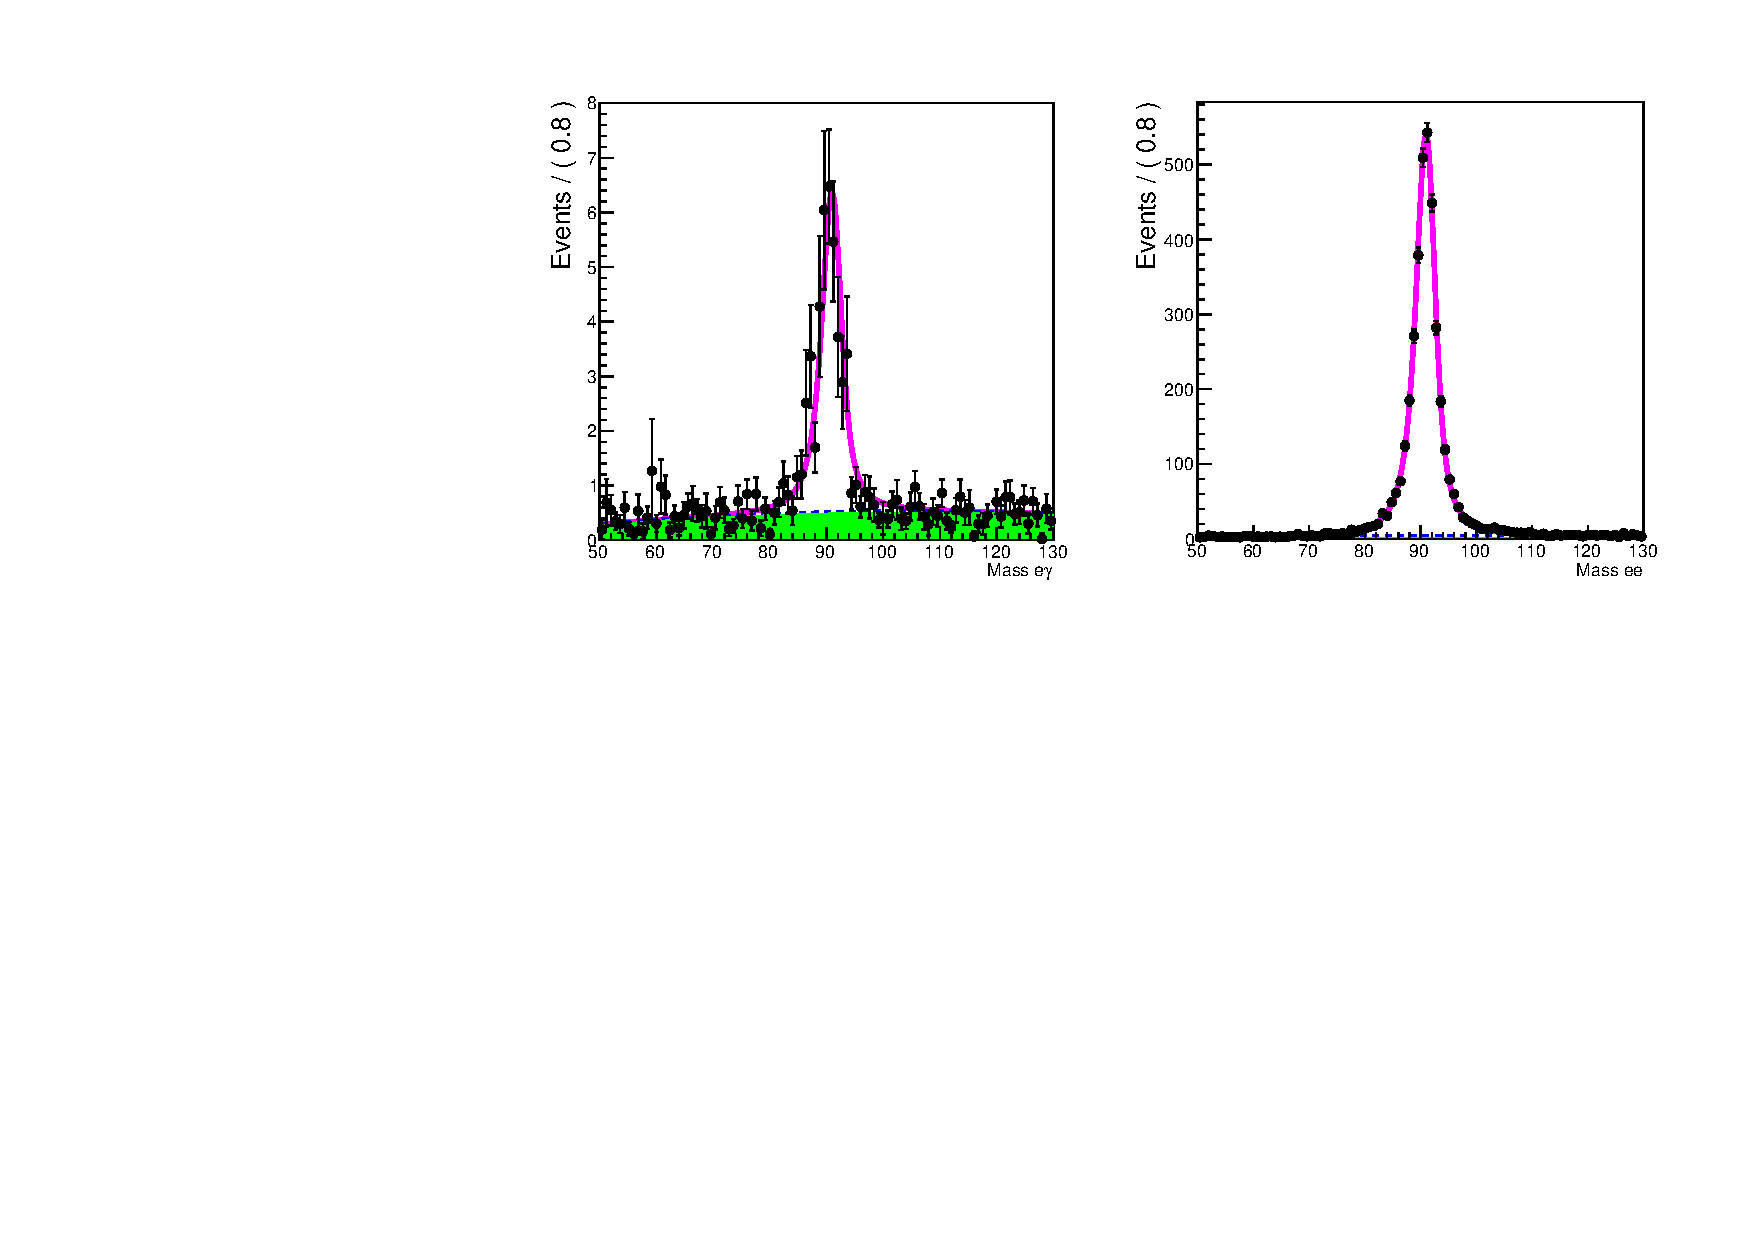
\includegraphics[width=0.48\linewidth]{../Figures/Chap3/fake_rate_tag_and_probe/tag_probe_MC_fit_qmult_0_1.pdf}
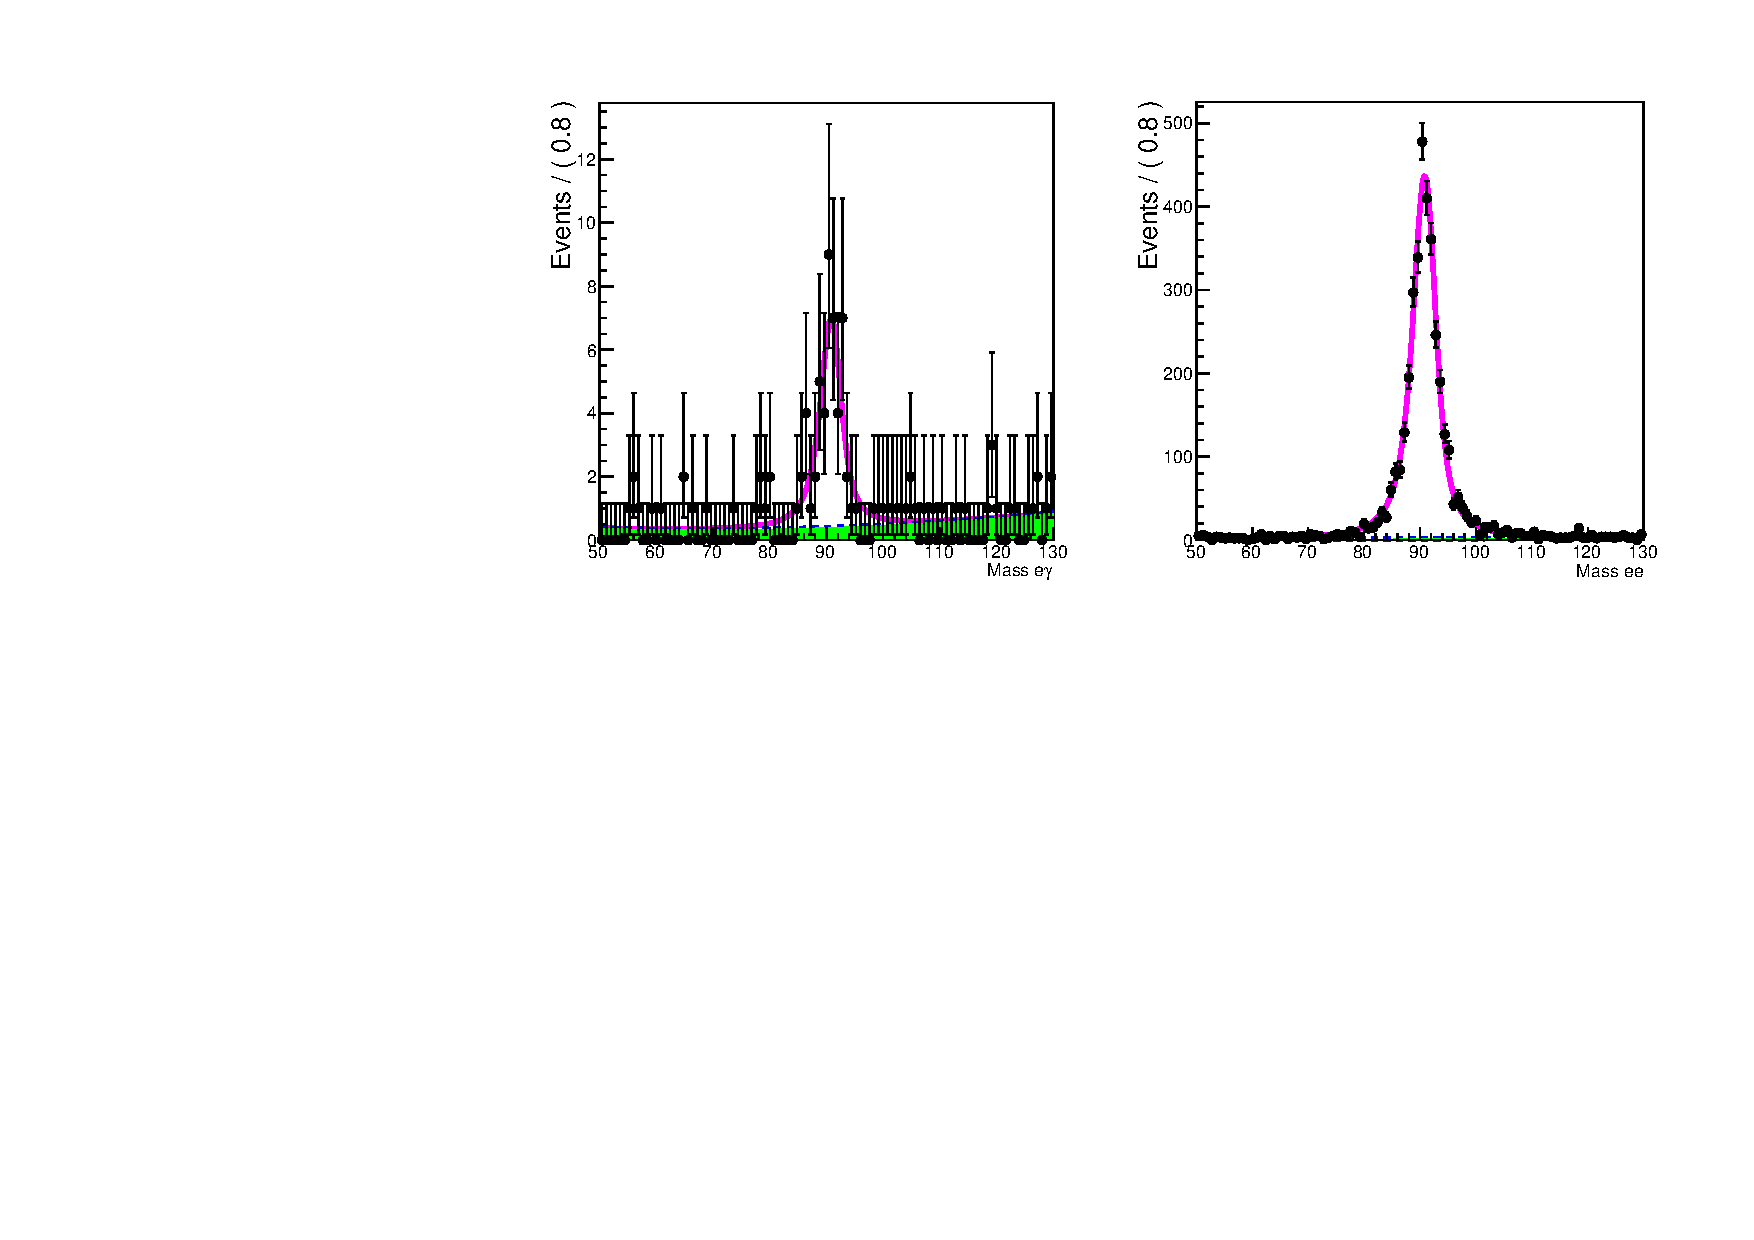
\includegraphics[width=0.48\linewidth]{../Figures/Chap3/fake_rate_tag_and_probe/tag_probe_fit_qmult_0_1.pdf}\\
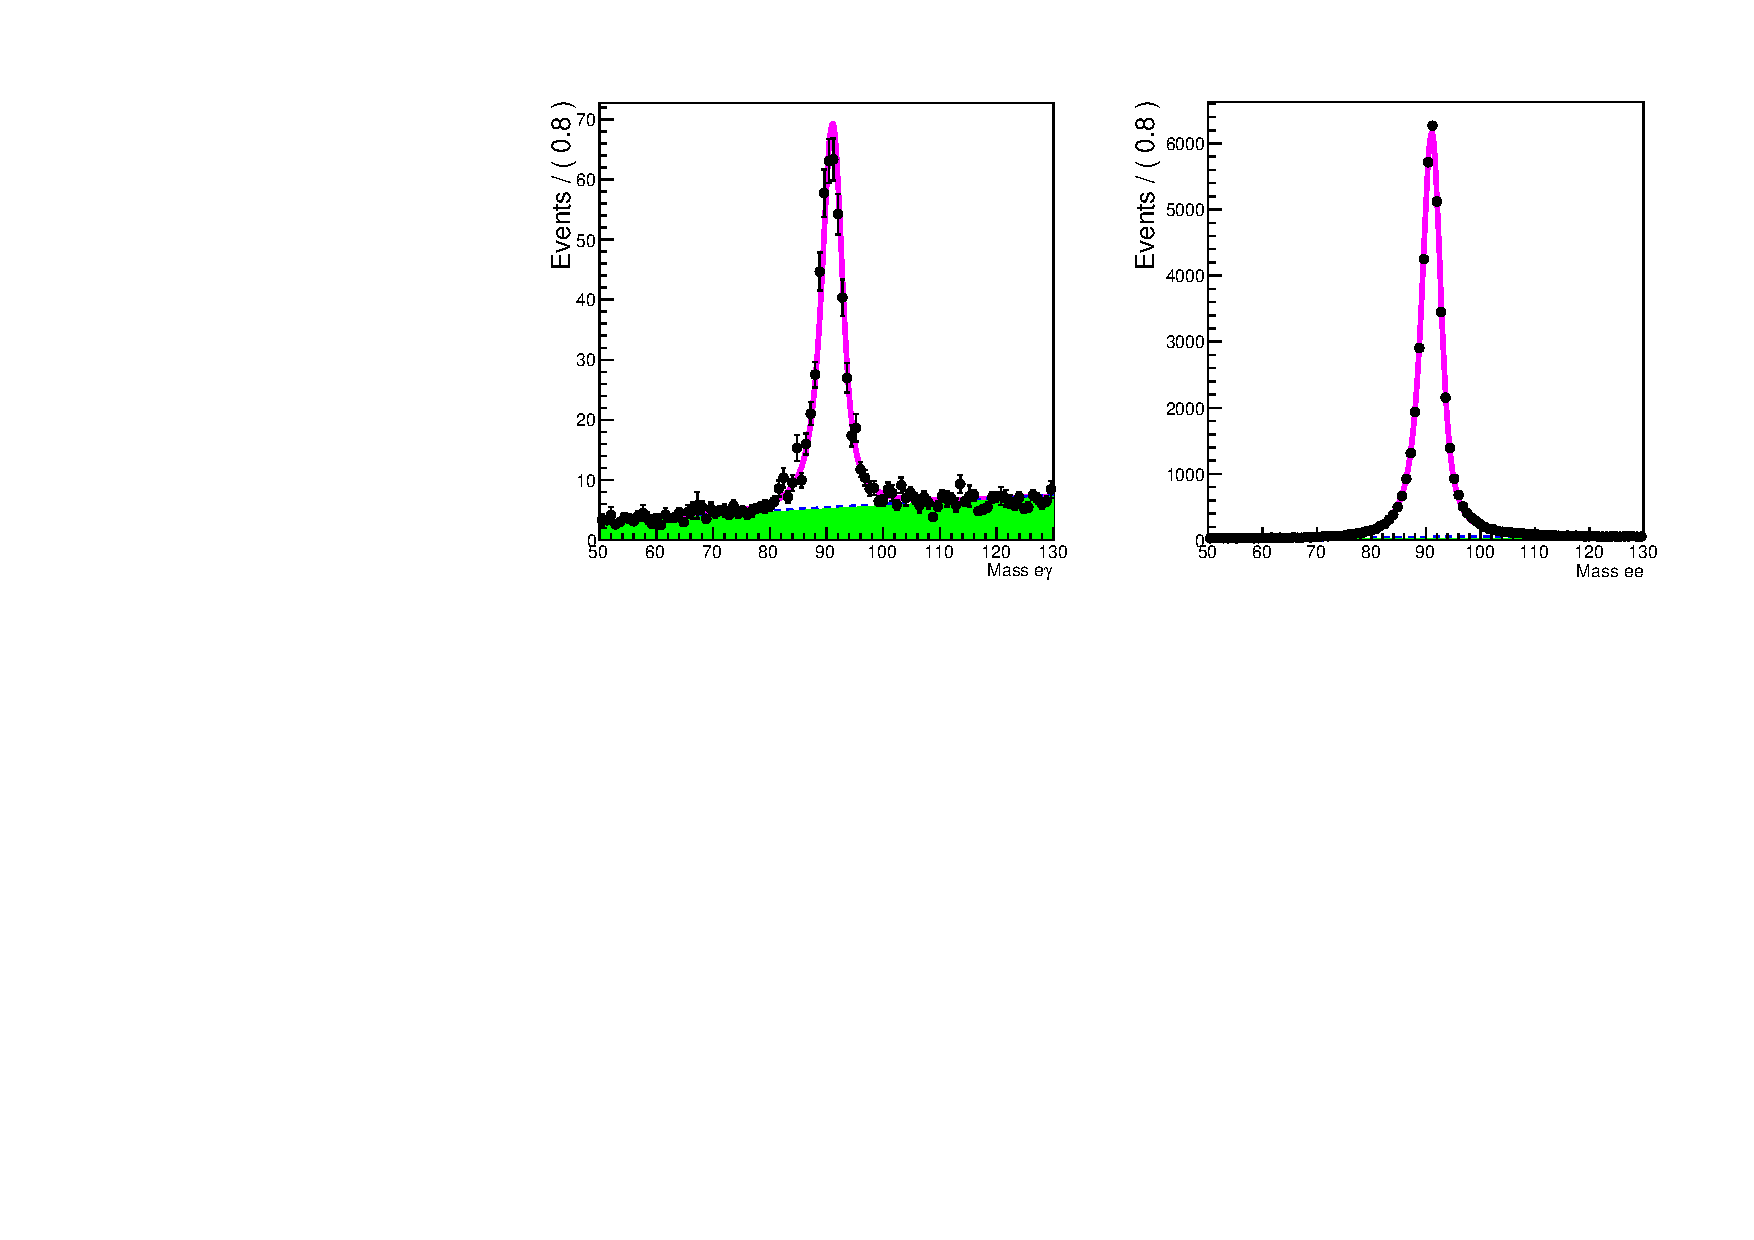
\includegraphics[width=0.48\linewidth]{../Figures/Chap3/fake_rate_tag_and_probe/tag_probe_MC_fit_qmult_2_100.pdf}
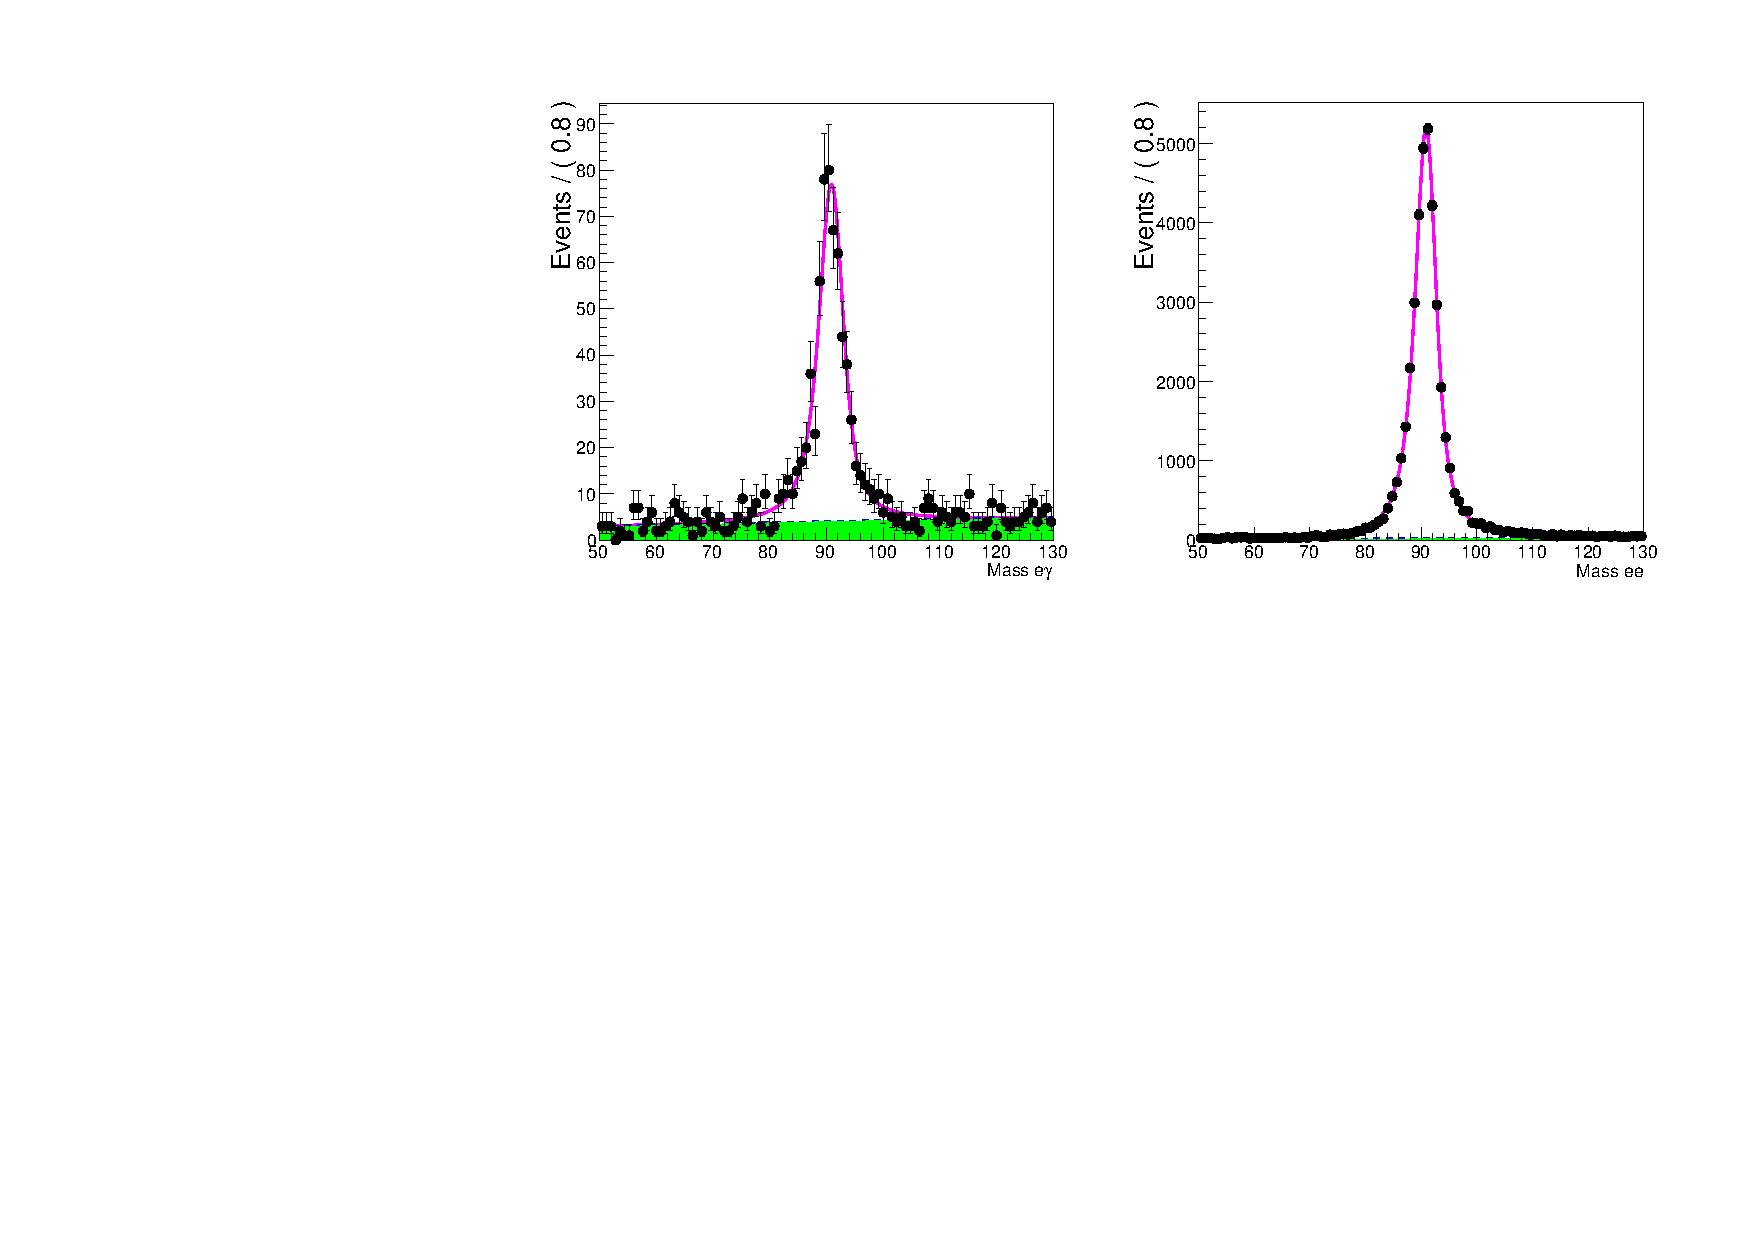
\includegraphics[width=0.48\linewidth]{../Figures/Chap3/fake_rate_tag_and_probe/tag_probe_fit_qmult_2_100.pdf}\\
\captionsetup{width=.9\linewidth}
\caption[Tag \& probe fits for data and MC]{Tag \& probe fits of the fake rate in 0-1 $Q_{mult}$ bins (top row) and $\geq2\ Q_{mult}$ bins (bottom row).
The first and second columns are the
the photon region and electron region fits in MC, respectively. The third and fourth columns are 
the photon region and electron region fits in data, respectively.}
\label{fig:tpFits}
\end{figure}

\subsubsection{Fake rate prediction}
Using the results described above, the prediction for the fake photon background is shown in 
Table~\ref{tab:fakeRatePredictions} (for high \dphi) and Table~\ref{tab:fakeRatePredictions_LDP} (for low \dphi).